\documentclass{beamer}
\usetheme{Copenhagen}
\usecolortheme{beaver}
\beamertemplatenavigationsymbolsempty
\makeatletter

\setbeamertemplate{footline}
{
  \leavevmode%
  \hbox{%
  \begin{beamercolorbox}[wd=.9\paperwidth,ht=2.25ex,dp=1ex,center]{author in head/foot}%
  \end{beamercolorbox}%
  \begin{beamercolorbox}[wd=.1\paperwidth,ht=2.25ex,dp=1ex,center]{title in head/foot}%
    \insertframenumber{} / 19
  \end{beamercolorbox}}%
  \vskip0pt%
}
\makeatother

\definecolor{unibored}{RGB}{187,46,41}
\setbeamercolor{title}{fg=unibored}
\setbeamercolor{beamercolorbox}{fg=unibored}

\setbeamertemplate{title page}{
    \vfill
    \begin{center}
        {\usebeamerfont{title}\usebeamercolor[fg]{title}\inserttitle\par}
    \end{center}

    \vfill

    \begin{center}
        {\usebeamerfont{author}\insertauthor\par}
        \vspace{0.2cm}
        {\usebeamerfont{institute}\insertinstitute\par}
        \vspace{0.5cm}
        {\usebeamerfont{date}\insertdate\par}
    \end{center}
}

\title{Merkle-tree-based integrity verification protocol for geo-distributed storage
systems}

\author{Presented by Santo Cariotti\\Supervised by Prof. Özalp Babaoğlu}

\institute{Alma Mater Studiorum\\ Università di Bologna}
\date{October 30, 2025}


\usepackage{listings}

\usepackage{graphicx}
\usepackage{tikz}
\usepackage{tikz-uml}
\usepackage{pgfplots}

\usetikzlibrary{arrows.meta,positioning,calc,fit}
\usetikzlibrary{shapes.geometric}
\usepackage[ruled,linesnumbered,vlined]{algorithm2e}
\usepackage{pgfplots,pgfplotstable}
\usepgfplotslibrary{groupplots}

\begin{document}

{
\setbeamertemplate{footline}{} 
\frame{\titlepage}
}

\addtocounter{framenumber}{-1}

% \begin{frame}{Content}

\begin{enumerate}
    \item<1-> What kind of problem are we facing?
    \item<2-> How did we manage to solve this?
    \item<3-> How about scalability?
\end{enumerate}

\end{frame}

\begin{frame}{Problem}
How can we verify that none of the files are corrupted?

\begin{center}
    \begin{tikzpicture}
        % 1. Include your image in a node
        \node[anchor=south west,inner sep=0] (image) at (0,0) {
            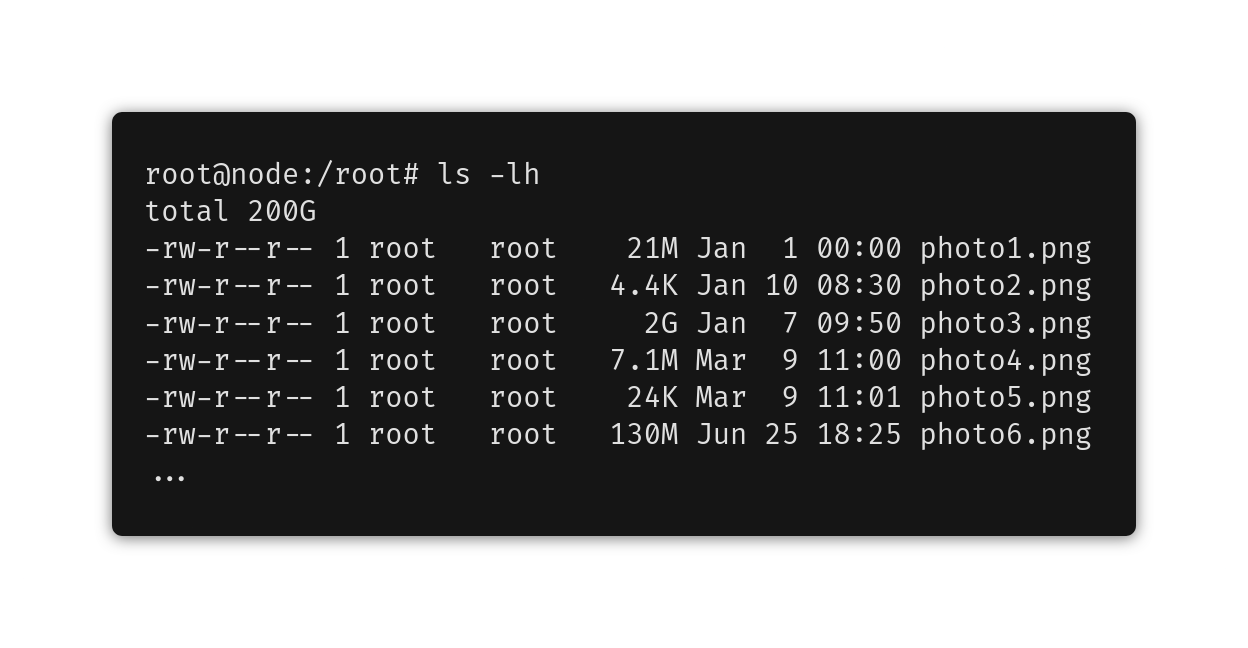
\includegraphics[width=0.8\linewidth]{static/shell-ls-problem.png}
        };

        % Calculate the width and height of the image node for later use
        \pgfgetlastxy{\imagewidth}{\imageheight}

        \coordinate (A) at ([xshift=.7cm, yshift=2.1cm]image.south west);
        \coordinate (B) at ([xshift=7.9cm, yshift=2.4cm]image.south west);

        \draw[red, very thick, line width=1pt]
            (A) rectangle (B);
    \end{tikzpicture}
\end{center}

We can use checksums.

\end{frame}

\begin{frame}{Problem}
    \begin{columns}[c]
        \begin{column}{0.4\textwidth}
            But, what if we have a file split in pieces and distributed across different regions?
            \only{We would need to perform a checksum on each node.}
        \end{column}
        \begin{column}{0.6\textwidth}

            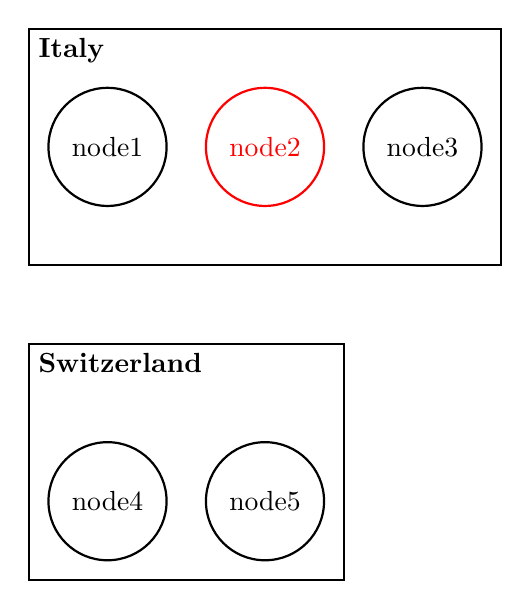
\begin{tikzpicture}
                \draw[thick] (0,0) rectangle (4,3);
                \node[anchor=north west] at (0,3) {\textbf{Switzerland}};
                \node[circle, draw, thick, minimum size=1.5cm] at (1,1) {node4};
                \node[circle, draw, thick, minimum size=1.5cm] at (3,1) {node5};

                \draw[thick] (0,4) rectangle (6,7);
                \node[anchor=north west] at (0,7) {\textbf{Italy}};
                \node[circle, draw, thick, minimum size=1.5cm] at (1,5.5) {node1};
                \node[circle, draw, red, thick, minimum size=1.5cm] at (3,5.5) {node2};
                \node[circle, draw, thick, minimum size=1.5cm] at (5,5.5) {node3};
            \end{tikzpicture}
        \end{column}
    \end{columns}
\end{frame}

\begin{frame}{Cubbit}
\centering

\includegraphics[width=0.4\linewidth]{static/cubbit-logo.png}
\\
\vspace{1em}
Cubbit, a geo-distributed storage system.\\
\end{frame}

\begin{frame}{Cubbit -- How it works}
    \begin{columns}[c]
        \begin{column}{0.4\textwidth}
            A file is split in $n+k$ shards. \\ We need at least $n$ shards to reconstruct the
            entire file, $k$ shards are used as redundancy.

        \end{column}
        \begin{column}{0.6\textwidth}

            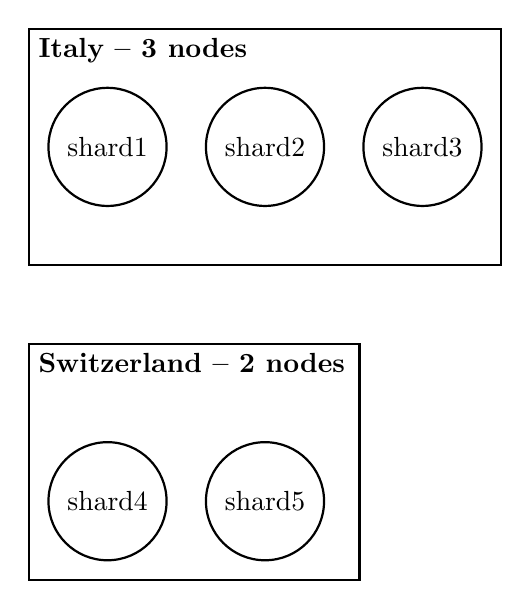
\begin{tikzpicture}
                \draw[thick] (0,0) rectangle (4.2,3);
                \node[anchor=north west] at (0,3) {\textbf{Switzerland -- 2 nodes}};
                \node[circle, draw, thick, minimum size=1.5cm] at (1,1) {shard4};
                \node[circle, draw, thick, minimum size=1.5cm] at (3,1) {shard5};

                \draw[thick] (0,4) rectangle (6,7);
                \node[anchor=north west] at (0,7) {\textbf{Italy -- 3 nodes}};
                \node[circle, draw, thick, minimum size=1.5cm] at (1,5.5) {shard1};
                \node[circle, draw, thick, minimum size=1.5cm] at (3,5.5) {shard2};
                \node[circle, draw, thick, minimum size=1.5cm] at (5,5.5) {shard3};
            \end{tikzpicture}
        \end{column}
    \end{columns}
\end{frame}

\begin{frame}{Cubbit -- Problems using checksum}
    \begin{columns}[c]
        \begin{column}{0.4\textwidth}
            \begin{enumerate}
                \item<1-> If nodes are offline, can't check all shards for a file.
                \item<2-> During an upload some agents can be offline, but they
                could be online during the check.
                \item<3-> Check for each reconstructed file or for each shard?
            \end{enumerate}

        \end{column}
        \begin{column}{0.6\textwidth}

            \begin{tikzpicture}
                \draw[thick] (0,0) rectangle (4.2,3);
                \node[anchor=north west] at (0,3) {\textbf{Switzerland -- 2 nodes}};
                \node[circle, draw, dotted, minimum size=1.5cm] at (1,1) {shard4};
                \node[circle, draw, dotted, minimum size=1.5cm] at (1,1) {shard4};
                \node[circle, draw, thick, minimum size=1.5cm] at (3,1) {shard5};

                \draw[thick] (0,4) rectangle (6,7);
                \node[anchor=north west] at (0,7) {\textbf{Italy -- 3 nodes}};
                \node[circle, draw, thick, minimum size=1.5cm] at (1,5.5) {shard1};
                \only<1>{\node[circle, draw, thick, minimum size=1.5cm] at (3,5.5) {shard2};}
                \only<2->{\node[circle, draw, thick, minimum size=1.5cm] at
                (3,5.5) {\textcolor{red}{n/a}};}
                \node[circle, draw, dotted, minimum size=1.5cm] at (5,5.5) {shard3};
            \end{tikzpicture}
        \end{column}
    \end{columns}
\end{frame}

\begin{frame}{Solution}

Each node uses a Merkle tree structure to organize shards during integrity verification.
All nodes agree on which file is corrupted through Raft consensus.
Data are organized using Reed-Solomon codes.

\begin{center}
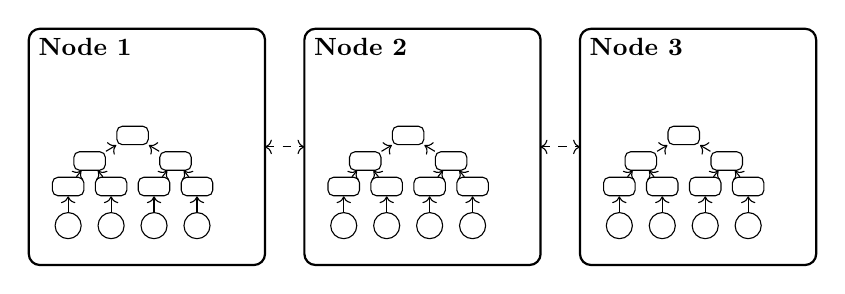
\begin{tikzpicture}[
    % Base styles for the small trees
    every node/.style={font=\small},
    leaf/.style={draw, circle, minimum size=2mm},
    hash/.style={draw, rectangle, rounded corners=2pt,
        minimum width=4mm, minimum height=2mm, % Increased size slightly
        sibling distance=1cm,
        align=center},
    node distance=2mm, % Increased distance slightly
    % Main positioning for the large blocks (not used as nodes, but kept)
    block/.style={draw, thick, rounded corners, inner sep=12pt}
]

% ==================== BLOCK 1: NODE 1 ====================
\begin{scope}[xshift=0cm]
    % leaves
    \node[leaf,] (d1-0) {};
    \node[leaf, right=of d1-0] (d1-1) {};
    \node[leaf, right=of d1-1] (d1-2) {};
    \node[leaf, right=of d1-2] (d1-3) {};
    % leaf-hash nodes
    \node[hash, above=0.2cm of d1-0] (n1-0) {};
    \node[hash, above=0.2cm of d1-1] (n1-1) {};
    \node[hash, above=0.2cm of d1-2] (n1-2) {};
    \node[hash, above=0.2cm of d1-3] (n1-3) {};
    % parents
    \node[hash, above=of $(n1-0)!0.5!(n1-1)$] (p1-01) {};
    \node[hash, above=of $(n1-2)!0.5!(n1-3)$] (p1-23) {};
    % root
    \node[hash, above=of $(p1-01)!0.5!(p1-23)$] (root1) {};
    % edges with arrows
    \foreach \a/\b in {d1-0/n1-0, d1-1/n1-1, d1-2/n1-2, d1-3/n1-3, n1-0/p1-01, n1-1/p1-01, n1-2/p1-23, n1-3/p1-23, p1-01/root1, p1-23/root1}
        \draw[->] (\a) -- (\b);

    % Explicitly drawn rectangle and label
    \draw[thick, rounded corners] (-0.5,-0.5) rectangle (2.5,2.5);
    \node[anchor=north west] at (-0.5,2.5) {\textbf{Node 1}};
    % Define coordinates for connection (center of the right edge)
    \coordinate (East1) at (2.5, 1.0); 
\end{scope}

% ==================== BLOCK 2: NODE 2 ====================
\begin{scope}[shift=({3.5cm, 0cm})]
    % leaves
    \node[leaf,] (d2-0) {};
    \node[leaf, right=of d2-0] (d2-1) {};
    \node[leaf, right=of d2-1] (d2-2) {};
    \node[leaf, right=of d2-2] (d2-3) {};
    % leaf-hash nodes
    \node[hash, above=0.2cm of d2-0] (n2-0) {};
    \node[hash, above=0.2cm of d2-1] (n2-1) {};
    \node[hash, above=0.2cm of d2-2] (n2-2) {};
    \node[hash, above=0.2cm of d2-3] (n2-3) {};
    % parents
    \node[hash, above=of $(n2-0)!0.5!(n2-1)$] (p2-01) {};
    \node[hash, above=of $(n2-2)!0.5!(n2-3)$] (p2-23) {};
    % root
    \node[hash, above=of $(p2-01)!0.5!(p2-23)$] (root2) {};
    % edges with arrows
    \foreach \a/\b in {d2-0/n2-0, d2-1/n2-1, d2-2/n2-2, d2-3/n2-3, n2-0/p2-01, n2-1/p2-01, n2-2/p2-23, n2-3/p2-23, p2-01/root2, p2-23/root2}
        \draw[->] (\a) -- (\b);

    % Explicitly drawn rectangle and label
    \draw[thick, rounded corners] (-0.5,-0.5) rectangle (2.5,2.5);
    \node[anchor=north west] at (-0.5,2.5) {\textbf{Node 2}};
    % Define coordinates for connection
    \coordinate (West2) at (-0.5, 1.0); % Left side center
    \coordinate (East2) at (2.5, 1.0);  % Right side center
\end{scope}

% ==================== BLOCK 3: NODE 3 ====================
\begin{scope}[shift=({7cm, 0cm})]
    % leaves
    \node[leaf,] (d3-0) {};
    \node[leaf, right=of d3-0] (d3-1) {};
    \node[leaf, right=of d3-1] (d3-2) {};
    \node[leaf, right=of d3-2] (d3-3) {};
    % leaf-hash nodes
    \node[hash, above=0.2cm of d3-0] (n3-0) {};
    \node[hash, above=0.2cm of d3-1] (n3-1) {};
    \node[hash, above=0.2cm of d3-2] (n3-2) {};
    \node[hash, above=0.2cm of d3-3] (n3-3) {};
    % parents
    \node[hash, above=of $(n3-0)!0.5!(n3-1)$] (p3-01) {};
    \node[hash, above=of $(n3-2)!0.5!(n3-3)$] (p3-23) {};
    % root
    \node[hash, above=of $(p3-01)!0.5!(p3-23)$] (root3) {};
    % edges with arrows
    \foreach \a/\b in {d3-0/n3-0, d3-1/n3-1, d3-2/n3-2, d3-3/n3-3, n3-0/p3-01, n3-1/p3-01, n3-2/p3-23, n3-3/p3-23, p3-01/root3, p3-23/root3}
        \draw[->] (\a) -- (\b);

    % Explicitly drawn rectangle and label
    \draw[thick, rounded corners] (-0.5,-0.5) rectangle (2.5,2.5);
    \node[anchor=north west] at (-0.5,2.5) {\textbf{Node 3}};
    % Define coordinates for connection
    \coordinate (West3) at (-0.5, 1.0); % Left side center
\end{scope}

% ==================== CONNECTIONS BETWEEN RECTANGLES ====================
% The coordinates are defined as global coordinates, so they can be referenced directly.
% Connection 1-2
\draw[<->, dashed] (East1) -- (West2);

% Connection 2-3
\draw[<->, dashed] (East2) -- (West3);

\end{tikzpicture}
\end{center}

\end{frame}


\begin{frame}
    \usebeamerfont{title}\usebeamercolor[fg]{title}Some background\par
\end{frame}

\begin{frame}{Merkle trees \only<2->{-- Proof}}
    \begin{columns}[c]
        \begin{column}{0.5\textwidth}
            \only<1>{It is a binary tree $T$ of height $H$ with $2^H$ leaves and
            $2^{H} - 1$ internal
nodes. Each leaf stores the cryptographic hash of the underlying data, rather than
the raw data itself. The same cryptographic hash function is applied recursively at
internal nodes, which store the hash of the concatenation of their two children.
            $$n_{parent} = f(n_{left} || n_{right})$$
            }
            \only<2>{Merkle trees has the ability to prove that a
given piece of data is part of a larger set, without revealing or recomputing the
            entire dataset. For $data_1$ we have $\pi=\{node_0, node_{23}\}$.}
            \only<3>{
Given a path $\pi$ we can make a proof verification
            comparing the result with the presumed root in $O(\log n)$.
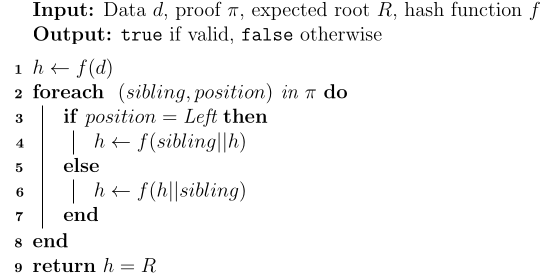
\includegraphics[width=1.1\linewidth]{static/merkle-proof-algorithm.png}
            }
        \end{column}
        \begin{column}{0.5\textwidth}
            \centering
            \begin{tikzpicture}[
              every node/.style={font=\tiny},
              leaf/.style={draw, circle, minimum size=7mm},
              hash/.style={draw, rectangle, rounded corners=2pt,
              minimum width=10mm, minimum height=7mm, 
              red/.style={draw=red},
              sibling distance=1cm,
              align=center},
              node distance=.6cm
            ]
            % leaves
            \node[leaf,] (data0) {$data_0$};
            \only<1>{\node[leaf, right=of data0] (data1) {$data_1$};}
            \only<2->{\node[leaf, red, right=of data0] (data1) {$data_1$};}
            \node[leaf, right=of data1] (data2) {$data_2$};
            \node[leaf, right=of data2] (data3) {$data_3$};
            % leaf-hash nodes with two lines (inline math for each line)
            \only<1>{\node[hash, above=0.2cm of data0] (n0) {\(\mathbf{node_0}\)\\ \(f(data_0)\)};}
            \only<2->{\node[hash, red, above=0.2cm of data0] (n0) {\(\mathbf{node_0}\)\\ \(f(data_0)\)};}
            \node[hash, above=0.2cm of data1] (n1) {\(\mathbf{node_1}\)\\ \(f(data_1)\)};
            \node[hash, above=0.2cm of data2] (n2) {\(\mathbf{node_2}\)\\ \(f(data_2)\)};
            \node[hash, above=0.2cm of data3] (n3) {\(\mathbf{node_3}\)\\ \(f(data_3)\)};
            % parents
            \node[hash, above=of $(n0)!0.5!(n1)$] (p01) {\(\mathbf{node_{01}}\)\\ \(f(node_0\Vert node_1)\)};
            \only<1>{\node[hash, above=of $(n2)!0.5!(n3)$] (p23) {\(\mathbf{node_{23}}\)\\ \(f(node_2\Vert node_3)\)};}
            \only<2->{\node[hash, red, above=of $(n2)!0.5!(n3)$] (p23) {\(\mathbf{node_{23}}\)\\ \(f(node_2\Vert node_3)\)};}
            % root
            \node[hash, above=of $(p01)!0.5!(p23)$] (root) {\(\textbf{root}\)\\ \(f(node_{01}\Vert node_{23})\)};
            % edges with arrows
            \foreach \a/\b in {data0/n0, data1/n1, data2/n2, data3/n3, n0/p01, n1/p01, n2/p23, n3/p23, p01/root, p23/root}
              \draw[->] (\a) -- (\b);
            \end{tikzpicture}
        \end{column}
    \end{columns}
\end{frame}

\begin{frame}{Raft}
A consensus protocol, where each server on a cluster is a follower, a candidate
or a leader. There is only leader and it is responsible to send messages to other servers via a log.

\centering

\includegraphics[width=.4\linewidth]{static/raft-logo.png}

\end{frame}

\begin{frame}{Reed-Solomon}

\only<1>{During an upload, a file is split in $n+k$ shards and send each
    shard to a different node.}
\only<2>{Up to $k$ agents could be offline, and the upload/download of files
    still works. We should make a recoverage of the missing shard when the agent
    comes back online.}

\vspace{1em}

\centering

\begin{tikzpicture}[
    % Set a global distance for 'right of' positioning
    node distance=1.5cm 
]

% Node 1: Start at (0,0)
\node[
    draw,
    cylinder,
    cylinder uses custom fill,
    cylinder body fill=gray!10,
    cylinder end fill=gray!40,
    minimum height=2.5cm,
    minimum width=1.5cm,
    align=center
] (C1) at (0,0) {Agent\\ 1};

% Node 2: Positioned to the right of Node 1
\only<1>{
    \node[
        draw,
        cylinder,
        cylinder uses custom fill,
        cylinder body fill=gray!10,
        cylinder end fill=gray!40,
        minimum height=2.5cm,
        minimum width=1.5cm,
        align=center,
        right=of C1 % <--- Positioning command
    ] (C2) {Agent\\ 2};
}

\only<2>{
    \node[
        draw,
        cylinder,
        cylinder uses custom fill,
        cylinder body fill=red!70,
        cylinder end fill=red!90,
        minimum height=2.5cm,
        minimum width=1.5cm,
        align=center,
        right=of C1 % <--- Positioning command
    ] (C2) {Agent\\ 2};
}

% Node 3: Positioned to the right of Node 2
\node[
    draw,
    cylinder,
    cylinder uses custom fill,
    cylinder body fill=gray!10,
    cylinder end fill=gray!40,
    minimum height=2.5cm,
    minimum width=1.5cm,
    align=center,
    right=of C2 % <--- Positioning command
] (C3) {Agent\\ 3};

\node[
    draw,
    circle,
    fill=blue!30,
    align=center,
    below=of C2 % <--- Positioning command
] (GW) {Gateway};


\draw[->, thick] (GW) -- (C1)
    node[midway, left, font=\scriptsize] {Shard 1};

\only<1>{\draw[->, thick] (GW) -- (C2)
     node[midway, left, font=\scriptsize] {Shard 2};}
\only<2>{\draw[->, red, thick] (GW) -- (C2)
    node[midway, left, font=\scriptsize] {Shard 2};}

\draw[->, thick] (GW) -- (C3)
    node[midway, right, font=\scriptsize] {Shard 3};

\end{tikzpicture}

\end{frame}

\begin{frame}
    \usebeamerfont{title}\usebeamercolor[fg]{title}Let's put all together\par
\end{frame}

\begin{frame}{Upload flow \only<6->{-- Directory tree}}
    Let's save our Christmas holidays family picture on Cubbit.
    \begin{itemize}
        \item<2-> Select a file. (e.g., xmas2024.png)
        \item<3-> Rename the file using a random string. (e.g., ff4c4b3)
        \item<4-> Use Reed-Solomon and send each shard to a different node. (e.g., ff4c4b3.1 to Agent 1)
        \item<5-> Store the file using a two-level of folders. (e.g. ff/4c/4b3.1 for Agent 1)
    \end{itemize}

    \only<6->{
        \begin{figure}[h]
        \centering
        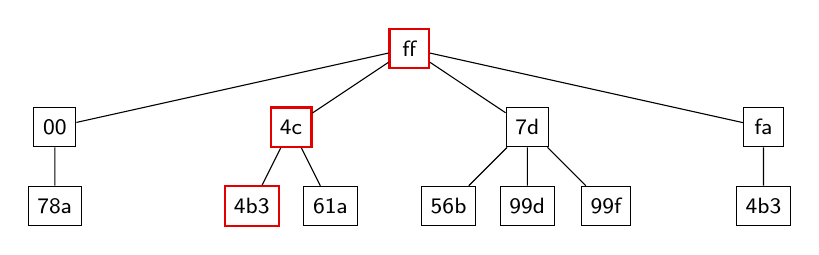
\begin{tikzpicture}[
          every node/.style={font=\sffamily\footnotesize, draw, rectangle, minimum size=5mm, align=center},
          level 1/.style={sibling distance=30mm, level distance=10mm},
          level 2/.style={sibling distance=10mm, level distance=10mm},
          red/.style={draw=red!90!black, thick},
          -, >=stealth
        ]

        \node[red] (root1) {ff}
            child {node {00}
              child {node {78a}}
            }
            child {node[red] {4c}
              child {node[red] {4b3}}
              child {node {61a}}
            }
            child {node {7d}
              child {node {56b}}
              child {node {99d}}
              child {node {99f}}
            }
            child {node {fa}
              child {node {4b3}}
            };
        \end{tikzpicture}
        \end{figure}
    }
\end{frame}

\begin{frame}{Directory trees as Merkle forest}

\begin{figure}
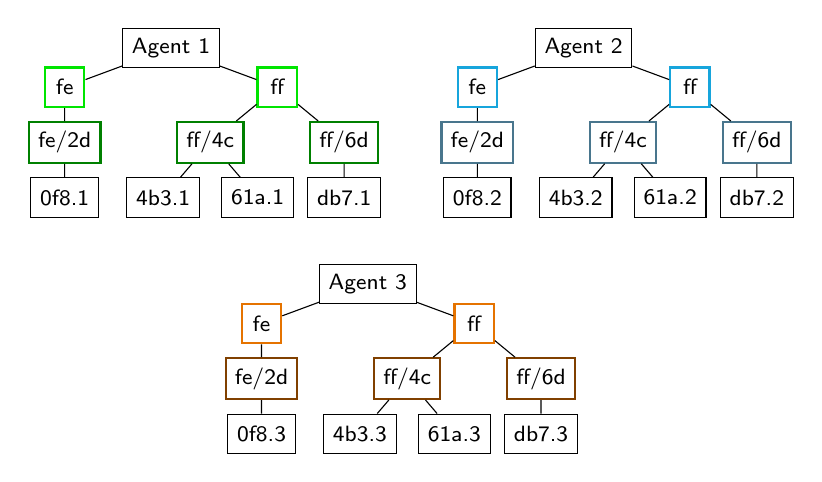
\begin{tikzpicture}[
  every node/.style={font=\sffamily\footnotesize, draw, rectangle, minimum size=5mm, align=center},
  greenborder/.style={draw=green!90!black, thick},
  greenborder2/.style={draw=green!50!black, thick},
  blueborder/.style={draw=cyan!90!black, thick},
  blueborder2/.style={draw=cyan!50!black, thick},
  yellowborder/.style={draw=orange!90!black, thick},
  yellowborder2/.style={draw=orange!50!black, thick},
  level 1/.style={sibling distance=27mm, level distance=5mm},
  level 2/.style={sibling distance=17mm, level distance=7mm},
  level 3/.style={sibling distance=12mm, level distance=7mm},
  -, >=stealth
]

\node (root1) {Agent 1}
  child {node[greenborder] {fe}
    child {node[greenborder2] {fe/2d}
      child {node {0f8.1}}
    }
  }
  child {node[greenborder] {ff}
    child {node[greenborder2] {ff/4c}
      child {node {4b3.1}}
      child {node {61a.1}}
    }
    child {node[greenborder2] {ff/6d}
      child {node {db7.1}}
    }
  };

\node[right=4cm of root1] (root2) {Agent 2}
  child {node[blueborder] {fe}
    child {node[blueborder2] {fe/2d}
      child {node {0f8.2}}
    }
  }
  child {node[blueborder] {ff}
    child {node[blueborder2] {ff/4c}
      child {node {4b3.2}}
      child {node {61a.2}}
    }
    child {node[blueborder2] {ff/6d}
      child {node {db7.2}}
    }
  };

\node (root3) at ($(root1) + (2.5cm,-3cm)$) {Agent 3}
  child {node[yellowborder] {fe}
    child {node[yellowborder2] {fe/2d}
      child {node {0f8.3}}
    }
  }
  child {node[yellowborder] {ff}
    child {node[yellowborder2] {ff/4c}
      child {node {4b3.3}}
      child {node {61a.3}}
    }
    child {node[yellowborder2] {ff/6d}
      child {node {db7.3}}
    }
  };

\end{tikzpicture}
\end{figure}

Every Agent sends Merkle tree root hashes for top-level and second-level folders to the Agent leader.

\end{frame}

\begin{frame}{Aggregated roots}


\begin{figure}[H]
\centering
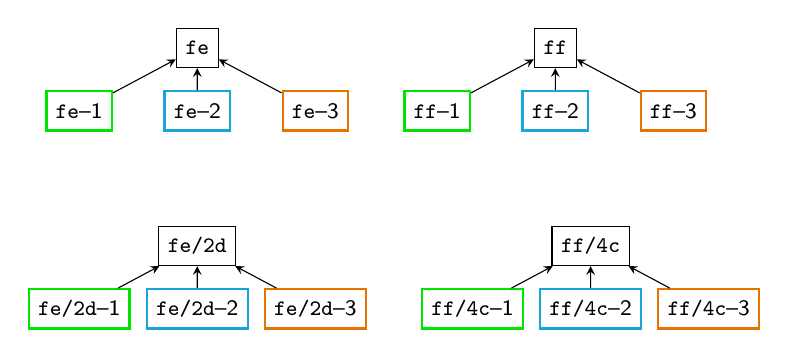
\begin{tikzpicture}[
  every node/.style={font=\sffamily\footnotesize, draw, rectangle, minimum size=5mm, align=center},
  hash1/.style={draw=green!90!black, thick},
  hash2/.style={draw=cyan!90!black, thick},
  hash3/.style={draw=orange!90!black, thick},
  level distance=8mm,
  sibling distance=15mm,
  <-, >=stealth
]

\node (fe) {\texttt{fe}}
  child {node[hash1] {\texttt{fe}--1}}
  child {node[hash2] {\texttt{fe}--2}}
  child {node[hash3] {\texttt{fe}--3}};

\node[right=4cm of fe] (ff) {\texttt{ff}}
  child {node[hash1] {\texttt{ff}--1}}
  child {node[hash2] {\texttt{ff}--2}}
  child {node[hash3] {\texttt{ff}--3}};

\node[below=2cm of fe](fe/2d) {\texttt{fe/2d}}
  child {node[hash1] {\texttt{fe/2d}--1}}
  child {node[hash2] {\texttt{fe/2d}--2}}
  child {node[hash3] {\texttt{fe/2d}--3}};

\node[right=4cm of fe/2d] (ff/4c) {\texttt{ff/4c}}
  child {node[hash1] {\texttt{ff/4c}--1}}
  child {node[hash2] {\texttt{ff/4c}--2}}
  child {node[hash3] {\texttt{ff/4c}--3}};

\end{tikzpicture}
\end{figure}

The Agent leader computes other Merkle trees for each folder using the Merkle tree hashes for
    each Agent.


\end{frame}


\begin{frame}[fragile]{Map of hashes}
\footnotesize
\begin{lstlisting}[language=Python, basicstyle=\ttfamily\footnotesize,
                   keywordstyle=\color{blue},
                   commentstyle=\color{gray},
                   stringstyle=\color{teal},
                   showstringspaces=false]
roots = {
    "fe":   "new root hash of fe",
    "ff":   "new root hash of ff",
    "ff/4c":"new root hash of ff/4c",
    # ...
}

agent_roots = {
    "fe": [
        "Agent 1 root hash of fe",
        "Agent 2 root hash of fe",
        "Agent 3 root hash of fe"
    ],
    # ...
    "ff/4c": [
        "Agent 1 root hash of ff/4c",
        "Agent 2 root hash of ff/4c",
        "Agent 3 root hash of ff/4c"
    ],
}
\end{lstlisting}
\end{frame}

\begin{frame}{Map of hashes}

This map allows us to:
\begin{itemize}
    \item Use \texttt{agent\_roots[<some\_folder>][i-th-agent]} when
        the i-th Agent is offline.
    \item If an Agent is offline during the upload, the
        \texttt{roots[<some\_folder>]} value is still computed using the
        current status of every Agent.
\end{itemize}

\end{frame}

\begin{frame}{Check corruptions}

\begin{figure}
\centering
\begin{tikzpicture}[scale=0.6, every node/.style={scale=0.8}]
\begin{umlseqdiag}

    % Define participants
    \umlobject[no ddots, x=0]{Agent 1}
    \umlobject[no ddots, x=9, fill=gray!20, draw=gray]{Agent 2}
    \umlobject[no ddots, x=14]{Agent 3}

    \only<2->{
        \begin{umlcall}[op=(1a) Get root hash for \texttt{ff}, dt=10, return=Root hash for \texttt{ff}]{Agent 1}{Agent 1}
        \end{umlcall}
    }

    \only<3->{
        \begin{umlcall}[op=(1b) Get root hash for Agent 2's \texttt{ff}, dt=10, return=\texttt{agent\_roots["ff"][2]}]{Agent 1}{Agent 1}
        \end{umlcall}
    }

    \only<4->{
        \begin{umlcall}[op=(1c) Get root hash for \texttt{ff}, dt=10, return=Root hash for \texttt{ff}]{Agent 1}{Agent 3}
        \end{umlcall}
    }

    \only<5->{
        \begin{umlcall}[op=(2a) Raft log with corruption status for \texttt{ff},
            fill=gray!10, dt=10]{Agent 1}{Agent 2}
        \end{umlcall}
        \begin{umlcall}[op=(2b) Raft log with corruption status for \texttt{ff}, fill=red, dt=10]{Agent 1}{Agent 3}
        \end{umlcall}
    }

\end{umlseqdiag}
\end{tikzpicture}
\end{figure}

\end{frame}

\begin{frame}{Tests -- Set up}
8 Agents with 4 CPU(s), 8-16 GB of RAM, and 45 GB of Disk.

\begin{center}
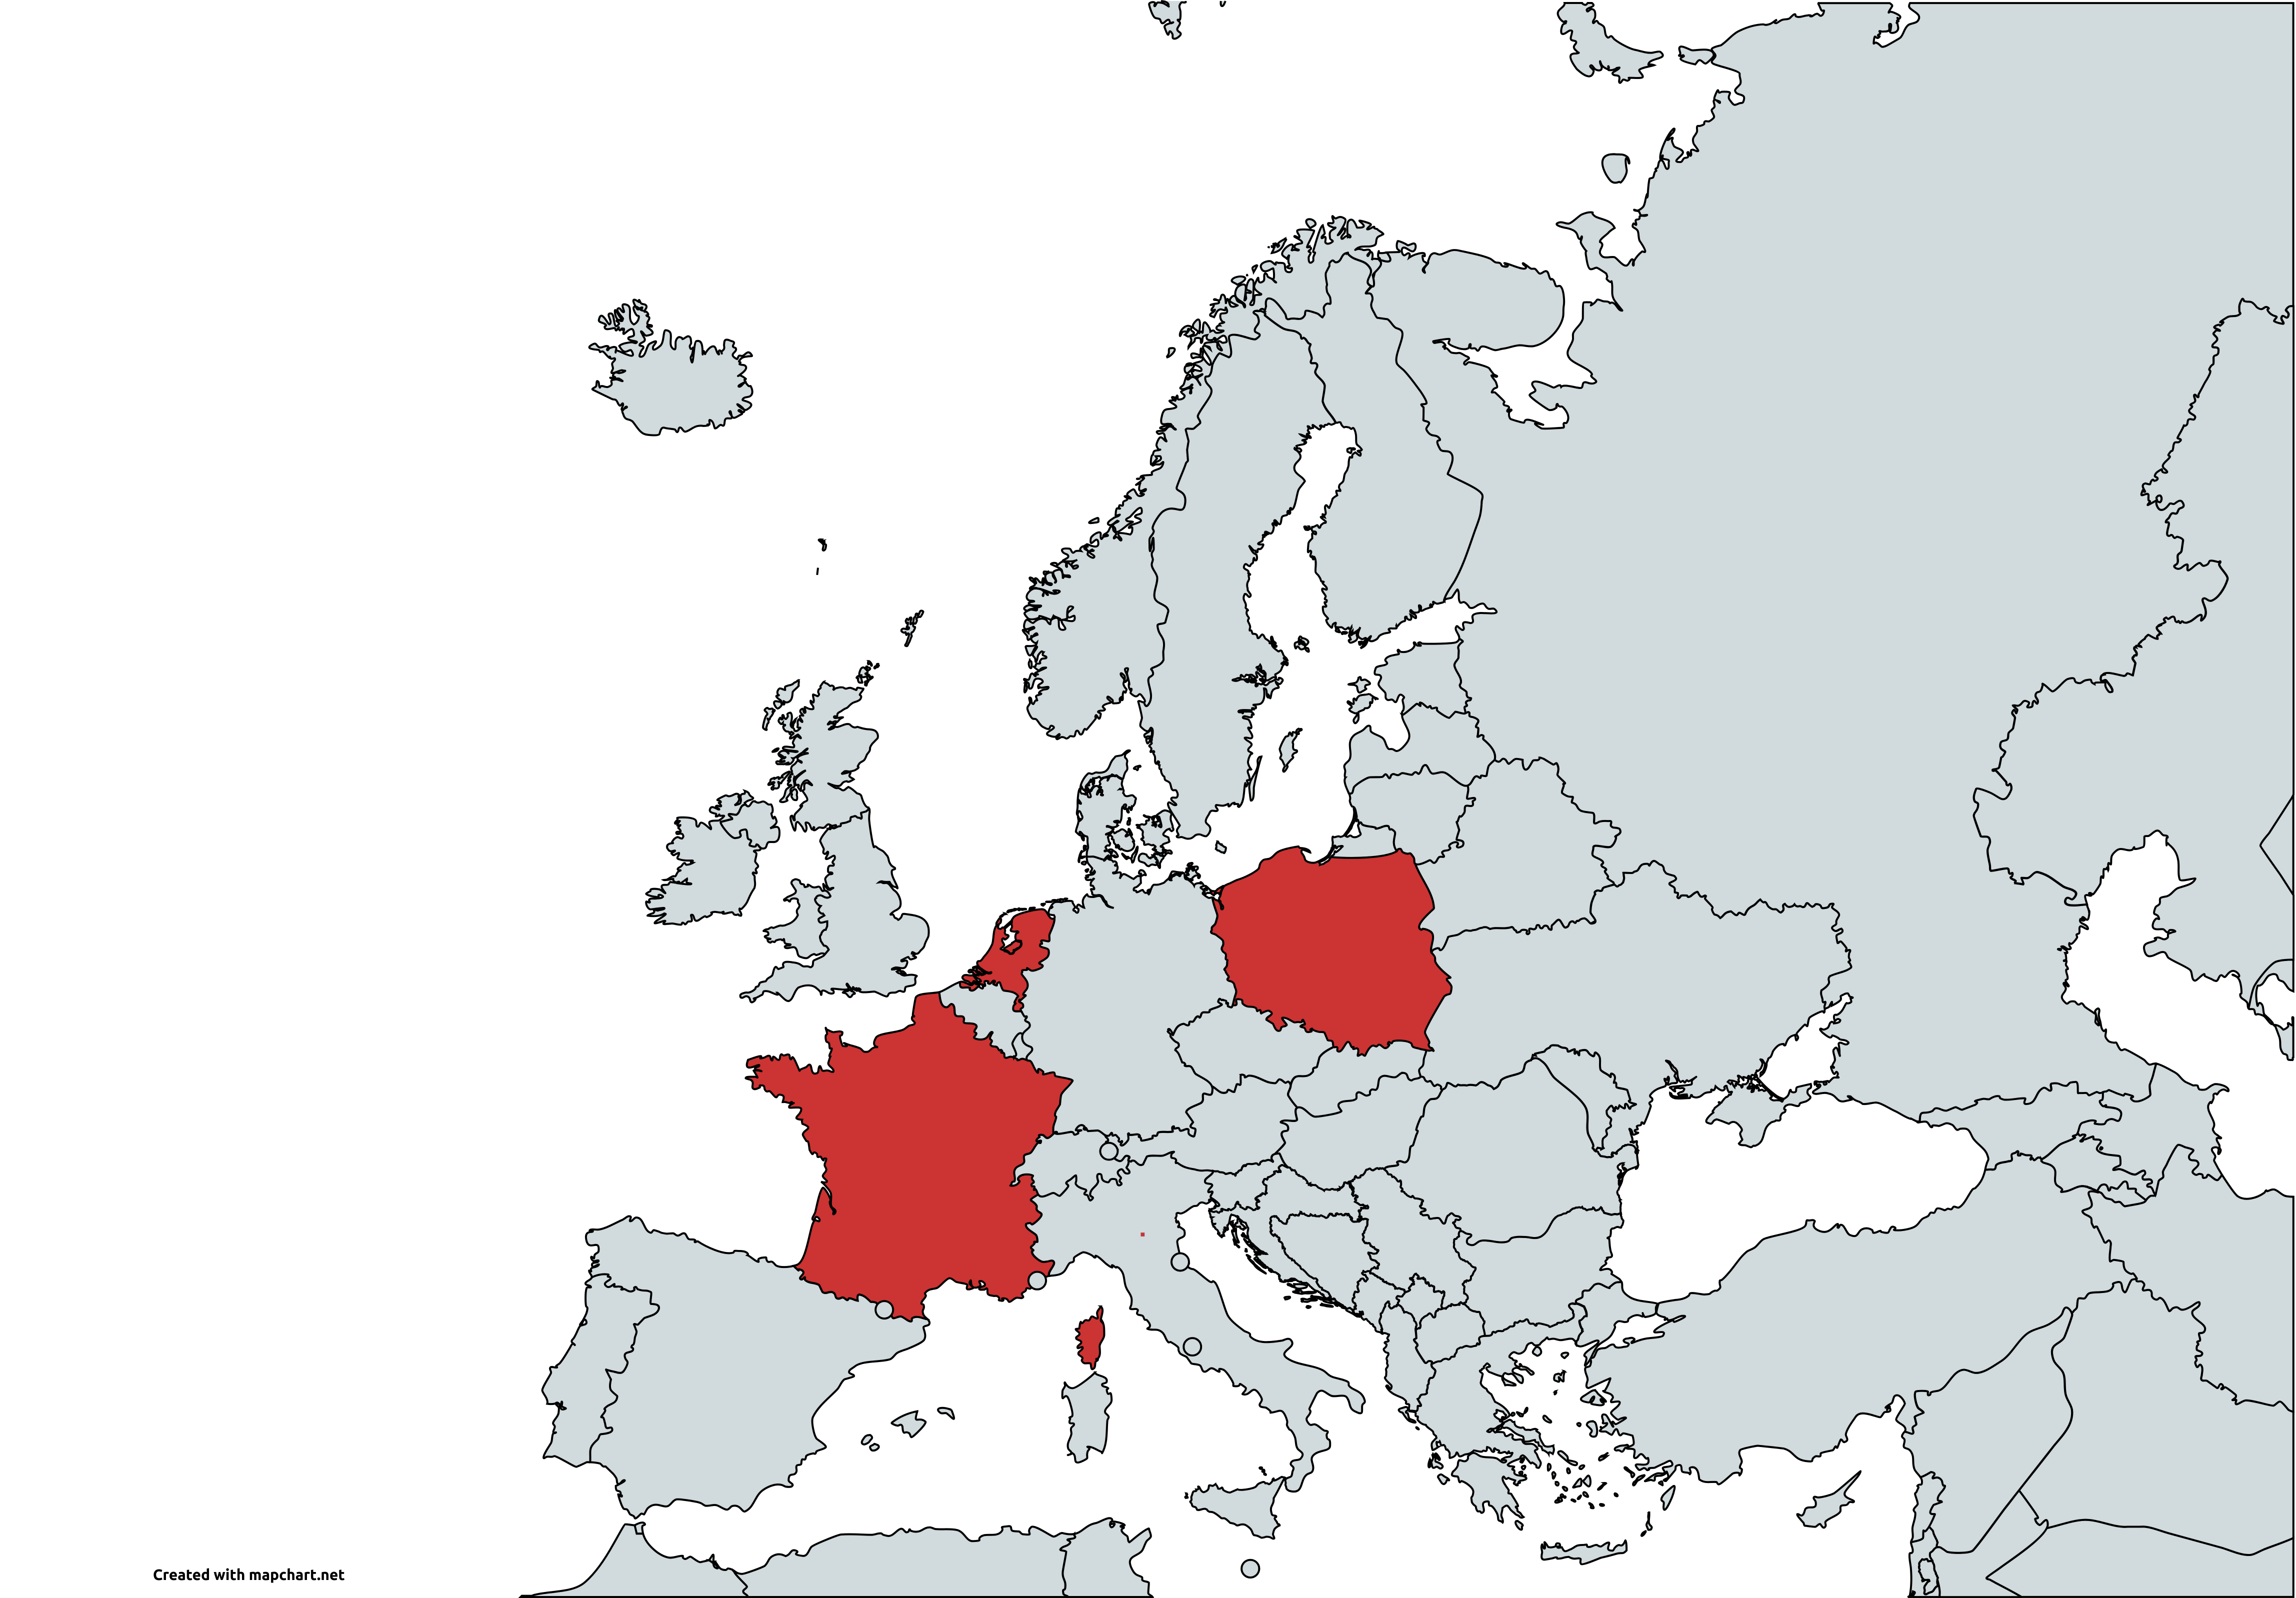
\includegraphics[width=0.5\linewidth]{static/map-chart.png}
\end{center}

For each test, we consider the number of online/offline agents and the file
    sizes and counts.

\end{frame}

\begin{frame}{Same dataset but different file size and count -- 1}

\begin{figure}
\centering
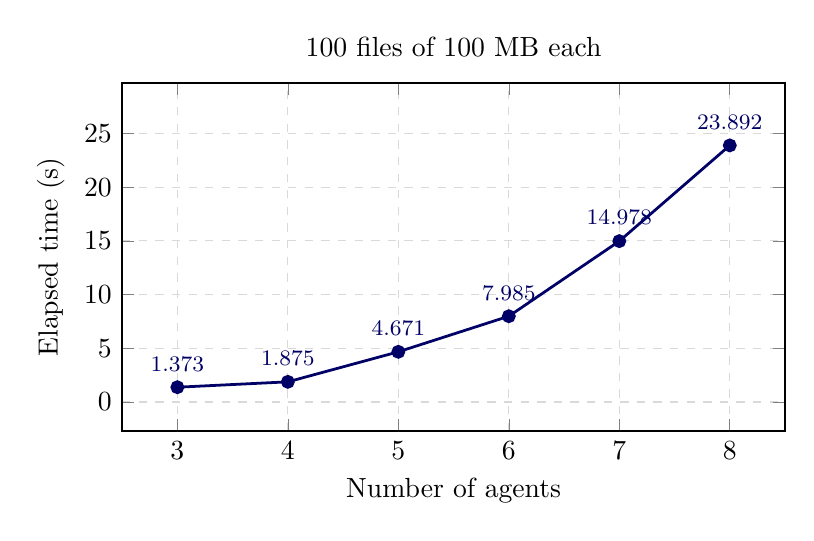
\begin{tikzpicture}
\begin{axis}[
    width=10cm, height=6cm,
    xlabel={Number of agents},
    ylabel={Elapsed time (s)},
    xmin=3, xmax=8,
    ymin=0, ymax=27,
    xtick={3,4,5,6,7,8},
    ytick={0,5,10,15,20,25},
    grid=major,
    grid style={dashed,gray!30},
    thick,
    title={100 files of 100 MB each},
    enlargelimits=0.1,
    clip=false,
    nodes near coords,
    every node near coord/.append style={font=\footnotesize, anchor=south, yshift=2pt},
    point meta=explicit symbolic
]

\addplot[color=blue!40!black, mark=*, line width=1pt] coordinates {
    (3,1.373) [1.373]
    (4,1.875) [1.875]
    (5,4.671) [4.671]
    (6,7.985) [7.985]
    (7,14.978) [14.978]
    (8,23.892) [23.892]
};
\end{axis}
\end{tikzpicture}
\end{figure}

\end{frame}

\begin{frame}{Same dataset but different file size and count -- 2}

\begin{figure}
\centering
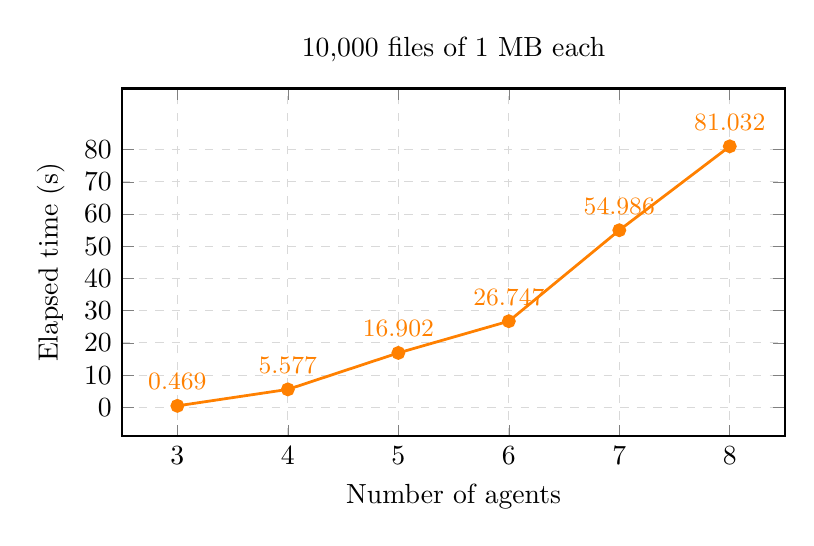
\begin{tikzpicture}
\begin{axis}[
    width=10cm, height=6cm,
    xlabel={Number of agents},
    ylabel={Elapsed time (s)},
    xmin=3, xmax=8,
    ymin=0, ymax=90,
    xtick={3,4,5,6,7,8},
    ytick={0,10,20,30,40,50,60,70,80},
    grid=major,
    grid style={dashed,gray!30},
    thick,
    title={10,000 files of 1 MB each},
    enlargelimits=0.1,
    clip=false,
    nodes near coords,
    every node near coord/.append style={font=\small, anchor=south, yshift=2pt},
    point meta=explicit symbolic
]

\addplot[color=orange, mark=*, line width=1pt] coordinates {
    (3,0.4685) [0.469]
    (4,5.577) [5.577]
    (5,16.902) [16.902]
    (6,26.747) [26.747]
    (7,54.986) [54.986]
    (8,81.032) [81.032]
};
\end{axis}
\end{tikzpicture}
\end{figure}

\end{frame}

\begin{frame}{Same dataset but different file size and count -- 3}

\begin{figure}
\centering
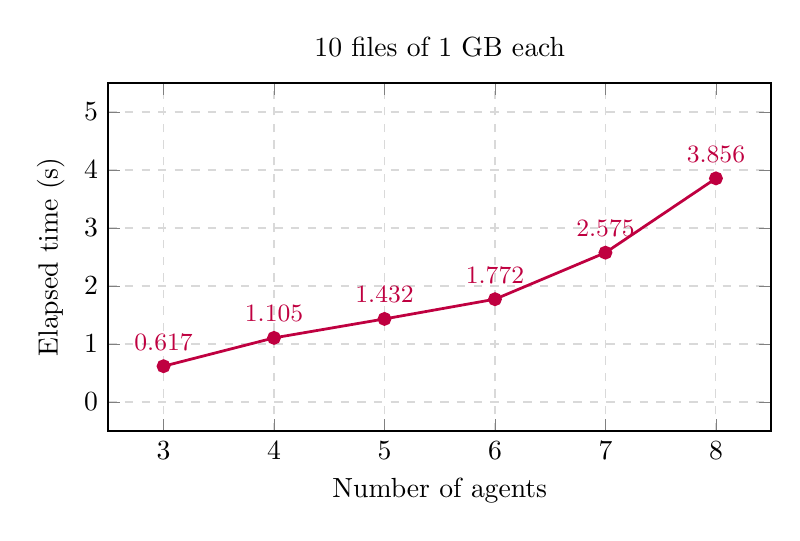
\begin{tikzpicture}
\begin{axis}[
    width=10cm, height=6cm,
    xlabel={Number of agents},
    ylabel={Elapsed time (s)},
    xmin=3, xmax=8,
    ymin=0, ymax=5,
    xtick={3,4,5,6,7,8},
    ytick={0,1,2,3,4,5},
    grid=major,
    grid style={dashed,gray!30},
    thick,
    title={10 files of 1 GB each},
    enlargelimits=0.1,
    clip=false,
    nodes near coords,
    every node near coord/.append style={font=\small, anchor=south, yshift=2pt},
    point meta=explicit symbolic
]

\addplot[color=purple, mark=*, line width=1pt] coordinates {
    (3,0.6166) [0.617]
    (4,1.105) [1.105]
    (5,1.432) [1.432]
    (6,1.772) [1.772]
    (7,2.575) [2.575]
    (8,3.856) [3.856]
};
\end{axis}
\end{tikzpicture}
\end{figure}

\end{frame}

\begin{frame}{Test with offline agents}

\begin{figure}
\centering
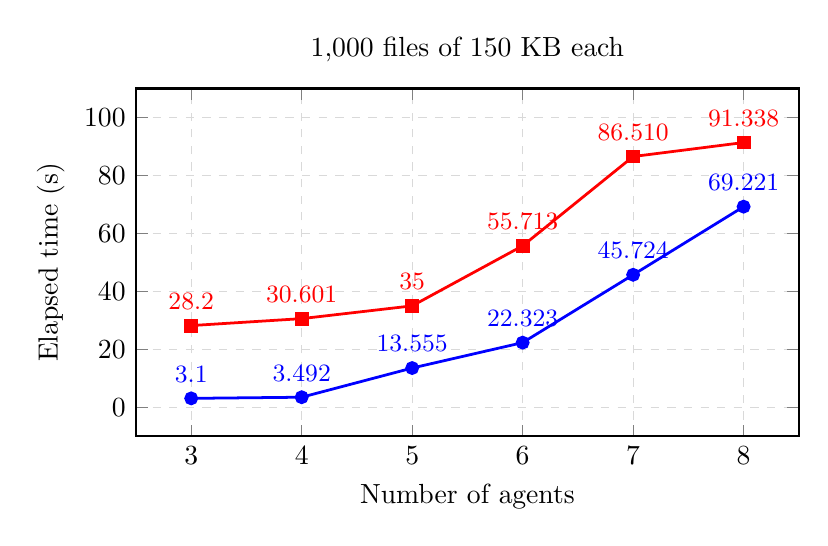
\begin{tikzpicture}
\begin{axis}[
    width=10cm, height=6cm,
    xlabel={Number of agents},
    ylabel={Elapsed time (s)},
    xmin=3, xmax=8,
    ymin=0, ymax=100,
    xtick={3,4,5,6,7,8},
    ytick={0,20,40,60,80,100},
    grid=major,
    grid style={dashed,gray!30},
    thick,
    title={1,000 files of 150 KB each},
    enlargelimits=0.1,
    clip=false,
    nodes near coords,
    every node near coord/.append style={font=\small, anchor=south, yshift=2pt},
    point meta=explicit symbolic
]

% Online agents
\addplot[color=blue, mark=*, line width=1pt] coordinates {
    (3,3.1) [3.1]
    (4,3.492) [3.492]
    (5,13.555) [13.555]
    (6,22.323) [22.323]
    (7,45.724) [45.724]
    (8,69.221) [69.221]
};

% Offline agents
\addplot[color=red, mark=square*, line width=1pt] coordinates {
    (3,28.2) [28.2]
    (4,30.601) [30.601]
    (5,35) [35]
    (6,55.713) [55.713]
    (7,86.510) [86.510]
    (8,91.338) [91.338]
};

\end{axis}
\end{tikzpicture}
\end{figure}

\end{frame}

\begin{frame}{Test with very large number of tiny files}

\begin{figure}
\centering
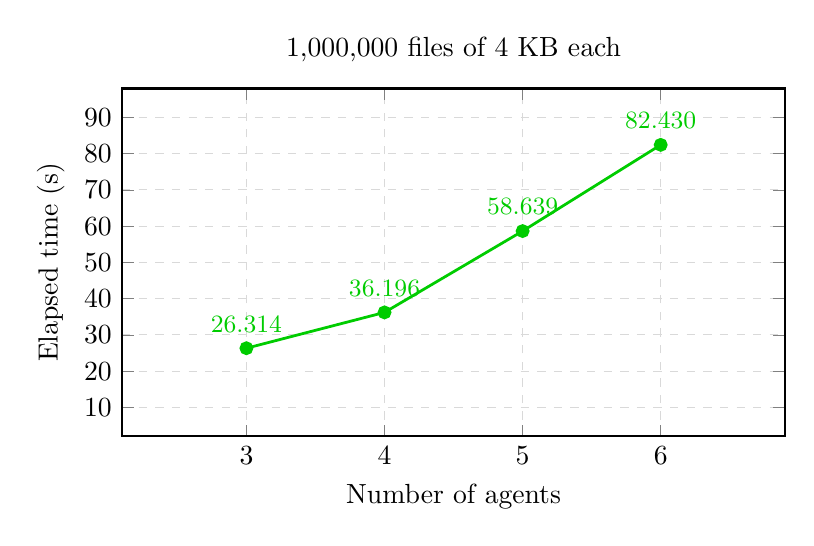
\begin{tikzpicture}
\begin{axis}[
    width=10cm, height=6cm,
    xlabel={Number of agents},
    ylabel={Elapsed time (s)},
    xmin=2.5, xmax=6.5,
    ymin=10, ymax=90,
    xtick={3,4,5,6},
    ytick={0,10,20,30,40,50,60,70,80,90,100},
    grid=major,
    grid style={dashed,gray!30},
    thick,
    title={1,000,000 files of 4 KB each},
    enlargelimits=0.1,
    clip=false,
    nodes near coords,
    every node near coord/.append style={font=\small, anchor=south, yshift=2pt},
    point meta=explicit symbolic
]

\addplot[color=green!80!black, mark=*, line width=1pt] coordinates {
    (3,26.314) [26.314]
    (4,36.196) [36.196]
    (5,58.639) [58.639]
    (6,82.430) [82.430]
};
\end{axis}
\end{tikzpicture}
\end{figure}

\end{frame}

\begin{frame}{Results}
\begin{itemize}
\item Scenarios with many small files amplify the cost of synchronization and consensus.
\item Verification time increases with the number of agents and files.
\item Confirmed the correctness and resilience of the approach under different scenarios and network conditions.
\end{itemize}
\end{frame}

\begin{frame}{Conclusion}

By combining Merkle trees, Raft consensus, and Reed-Solomon codes, we built a scalable and fault-tolerant protocol for distributed data integrity verification without relying on full file scans or constant node availability.
\end{frame}


\begin{frame}
\centering
    \usebeamerfont{title}\usebeamercolor[fg]{title}Thank you\par
\end{frame}


\end{document}
